%%%%%%%%%%%%%%%%%%%%%%%%%%%%%%%%%%%%%%%%%
% Masters/Doctoral Thesis 
% LaTeX Template
% Version 2.3 (25/3/16)
%
% This template has been downloaded from:
% http://www.LaTeXTemplates.com
%
% Version 2.x major modifications by:
% Vel (vel@latextemplates.com)
%
% This template is based on a template by:
% Steve Gunn (http://users.ecs.soton.ac.uk/srg/softwaretools/document/templates/)
% Sunil Patel (http://www.sunilpatel.co.uk/thesis-template/)
%
% Template license:
% CC BY-NC-SA 3.0 (http://creativecommons.org/licenses/by-nc-sa/3.0/)
%
%%%%%%%%%%%%%%%%%%%%%%%%%%%%%%%%%%%%%%%%%

%----------------------------------------------------------------------------------------
%	PACKAGES AND OTHER DOCUMENT CONFIGURATIONS
%----------------------------------------------------------------------------------------

\documentclass[
11pt, % The default document font size, options: 10pt, 11pt, 12pt
%oneside, % Two side (alternating margins) for binding by default, uncomment to switch to one side
%chapterinoneline,% Have the chapter title next to the number in one single line
english, % ngerman for German
singlespacing, % Single line spacing, alternatives: onehalfspacing or doublespacing
%draft, % Uncomment to enable draft mode (no pictures, no links, overfull hboxes indicated)
%nolistspacing, % If the document is onehalfspacing or doublespacing, uncomment this to set spacing in lists to single
%liststotoc, % Uncomment to add the list of figures/tables/etc to the table of contents
%toctotoc, % Uncomment to add the main table of contents to the table of contents
%parskip, % Uncomment to add space between paragraphs
%nohyperref, % Uncomment to not load the hyperref package
headsepline, % Uncomment to get a line under the header
]{MastersDoctoralThesis} % The class file specifying the document structure

\usepackage[utf8]{inputenc} % Required for inputting international characters
\usepackage[T1]{fontenc} % Output font encoding for international characters

\usepackage{palatino} % Use the Palatino font by default

\usepackage[backend=bibtex,style=authoryear,natbib=true]{biblatex} % Use the bibtex backend with the authoryear citation style (which resembles APA)

\addbibresource{example.bib} % The filename of the bibliography

\usepackage[autostyle=true]{csquotes} % Required to generate language-dependent quotes in the bibliography

%----------------------------------------------------------------------------------------
%	MARGIN SETTINGS
%----------------------------------------------------------------------------------------

\geometry{
	paper=a4paper, % Change to letterpaper for US letter
	inner=2.5cm, % Inner margin
	outer=3.8cm, % Outer margin
	bindingoffset=2cm, % Binding offset
	top=1.5cm, % Top margin
	bottom=1.5cm, % Bottom margin
	%showframe,% show how the type block is set on the page
}

%----------------------------------------------------------------------------------------
%	THESIS INFORMATION
%----------------------------------------------------------------------------------------

\thesistitle{Thesis Title} % Your thesis title, this is used in the title and abstract, print it elsewhere with \ttitle
\supervisor{Dr. James \textsc{Smith}} % Your supervisor's name, this is used in the title page, print it elsewhere with \supname
\examiner{} % Your examiner's name, this is not currently used anywhere in the template, print it elsewhere with \examname
\degree{Doctor of Philosophy} % Your degree name, this is used in the title page and abstract, print it elsewhere with \degreename
\author{John \textsc{Smith}} % Your name, this is used in the title page and abstract, print it elsewhere with \authorname
\addresses{} % Your address, this is not currently used anywhere in the template, print it elsewhere with \addressname

\subject{Biological Sciences} % Your subject area, this is not currently used anywhere in the template, print it elsewhere with \subjectname
\keywords{} % Keywords for your thesis, this is not currently used anywhere in the template, print it elsewhere with \keywordnames
\university{\href{http://www.university.com}{University Name}} % Your university's name and URL, this is used in the title page and abstract, print it elsewhere with \univname
\department{\href{http://department.university.com}{Department or School Name}} % Your department's name and URL, this is used in the title page and abstract, print it elsewhere with \deptname
\group{\href{http://researchgroup.university.com}{Research Group Name}} % Your research group's name and URL, this is used in the title page, print it elsewhere with \groupname
\faculty{\href{http://faculty.university.com}{Faculty Name}} % Your faculty's name and URL, this is used in the title page and abstract, print it elsewhere with \facname

\hypersetup{pdftitle=\ttitle} % Set the PDF's title to your title
\hypersetup{pdfauthor=\authorname} % Set the PDF's author to your name
\hypersetup{pdfkeywords=\keywordnames} % Set the PDF's keywords to your keywords

\begin{document}

\frontmatter % Use roman page numbering style (i, ii, iii, iv...) for the pre-content pages

\pagestyle{plain} % Default to the plain heading style until the thesis style is called for the body content

%----------------------------------------------------------------------------------------
%	TITLE PAGE
%----------------------------------------------------------------------------------------

\begin{titlepage}
\begin{center}

{\scshape\LARGE \univname\par}\vspace{1.5cm} % University name
\textsc{\Large Doctoral Thesis}\\[0.5cm] % Thesis type

\HRule \\[0.4cm] % Horizontal line
{\huge \bfseries \ttitle\par}\vspace{0.4cm} % Thesis title
\HRule \\[1.5cm] % Horizontal line
 
\begin{minipage}[t]{0.4\textwidth}
\begin{flushleft} \large
\emph{Author:}\\
\href{http://www.johnsmith.com}{\authorname} % Author name - remove the \href bracket to remove the link
\end{flushleft}
\end{minipage}
\begin{minipage}[t]{0.4\textwidth}
\begin{flushright} \large
\emph{Supervisor:} \\
\href{http://www.jamessmith.com}{\supname} % Supervisor name - remove the \href bracket to remove the link  
\end{flushright}
\end{minipage}\\[3cm]
 
\large \textit{A thesis submitted in fulfillment of the requirements\\ for the degree of \degreename}\\[0.3cm] % University requirement text
\textit{in the}\\[0.4cm]
\groupname\\\deptname\\[2cm] % Research group name and department name
 
{\large \today}\\[4cm] % Date
%\includegraphics{Logo} % University/department logo - uncomment to place it
 
\vfill
\end{center}
\end{titlepage}

%----------------------------------------------------------------------------------------
%	DECLARATION PAGE
%----------------------------------------------------------------------------------------

\begin{declaration}
\addchaptertocentry{\authorshipname}

\noindent I, \authorname, declare that this thesis titled, \enquote{\ttitle} and the work presented in it are my own. I confirm that:

\begin{itemize} 
\item This work was done wholly or mainly while in candidature for a research degree at this University.
\item Where any part of this thesis has previously been submitted for a degree or any other qualification at this University or any other institution, this has been clearly stated.
\item Where I have consulted the published work of others, this is always clearly attributed.
\item Where I have quoted from the work of others, the source is always given. With the exception of such quotations, this thesis is entirely my own work.
\item I have acknowledged all main sources of help.
\item Where the thesis is based on work done by myself jointly with others, I have made clear exactly what was done by others and what I have contributed myself.\\
\end{itemize}
 
\noindent Signed:\\
\rule[0.5em]{25em}{0.5pt} % This prints a line for the signature
 
\noindent Date:\\
\rule[0.5em]{25em}{0.5pt} % This prints a line to write the date
\end{declaration}

\cleardoublepage

%----------------------------------------------------------------------------------------
%	QUOTATION PAGE
%----------------------------------------------------------------------------------------

\vspace*{0.2\textheight}

\noindent\enquote{\itshape Thanks to my solid academic training, today I can write hundreds of words on virtually any topic without possessing a shred of information, which is how I got a good job in journalism.}\bigbreak

\hfill Dave Barry

%----------------------------------------------------------------------------------------
%	ABSTRACT PAGE
%----------------------------------------------------------------------------------------

\begin{abstract}
\addchaptertocentry{\abstractname} % Add the abstract to the table of contents

The Thesis Abstract is written here (and usually kept to just this page). The page is kept centered vertically so can expand into the blank space above the title too\ldots

\end{abstract}

%----------------------------------------------------------------------------------------
%	ACKNOWLEDGEMENTS
%----------------------------------------------------------------------------------------

\begin{acknowledgements}
\addchaptertocentry{\acknowledgementname} % Add the acknowledgements to the table of contents

The acknowledgments and the people to thank go here, don't forget to include your project advisor\ldots

\end{acknowledgements}

%----------------------------------------------------------------------------------------
%	LIST OF CONTENTS/FIGURES/TABLES PAGES
%----------------------------------------------------------------------------------------

%\tableofcontents % Prints the main table of contents

%\listoffigures % Prints the list of figures

%\listoftables % Prints the list of tables

%----------------------------------------------------------------------------------------
%	ABBREVIATIONS
%----------------------------------------------------------------------------------------

%\begin{abbreviations}{ll} % Include a list of abbreviations (a table of two columns)

%\textbf{LAH} & \textbf{L}ist \textbf{A}bbreviations \textbf{H}ere\\
%\textbf{WSF} & \textbf{W}hat (it) \textbf{S}tands \textbf{F}or\\

%\end{abbreviations}

%----------------------------------------------------------------------------------------
%	PHYSICAL CONSTANTS/OTHER DEFINITIONS
%----------------------------------------------------------------------------------------

%\begin{constants}{lr@{${}={}$}l} % The list of physical constants is a three column table

% The \SI{}{} command is provided by the siunitx package, see its documentation for instructions on how to use it

%	Speed of Light & $c_{0}$ & \SI{2.99792458e8}{\meter\per\second} (exact)\\
%Constant Name & $Symbol$ & $Constant Value$ with units\\

%\end{constants}

%----------------------------------------------------------------------------------------
%	SYMBOLS
%----------------------------------------------------------------------------------------

%\begin{symbols}{lll} % Include a list of Symbols (a three column table)

%$a$ & distance & \si{\meter} \\
%$P$ & power & \si{\watt} (\si{\joule\per\second}) \\
%Symbol & Name & Unit \\

%\addlinespace % Gap to separate the Roman symbols from the Greek

%$\omega$ & angular frequency & \si{\radian} \\

%\end{symbols}

%----------------------------------------------------------------------------------------
%	DEDICATION
%----------------------------------------------------------------------------------------

\dedicatory{For/Dedicated to/To my\ldots} 

%----------------------------------------------------------------------------------------
%	THESIS CONTENT - CHAPTERS
%----------------------------------------------------------------------------------------

\mainmatter % Begin numeric (1,2,3...) page numbering

\pagestyle{thesis} % Return the page headers back to the "thesis" style

% Include the chapters of the thesis as separate files from the Chapters folder
% Uncomment the lines as you write the chapters

% Chapter 1

\chapter[Motivation and Background]
{Motivation and Background} % Main chapter title

\label{Chapter1} % For referencing the chapter elsewhere, use \ref{Chapter1} 

%----------------------------------------------------------------------------------------






% Define some commands to keep the formatting separated from the content 
\newcommand{\keyword}[1]{\textbf{#1}}
\newcommand{\tabhead}[1]{\textbf{#1}}
\newcommand{\code}[1]{\texttt{#1}}
\newcommand{\file}[1]{\texttt{\bfseries#1}}
\newcommand{\option}[1]{\texttt{\itshape#1}}

%----------------------------------------------------------------------------------------

\section[Quantum info processing and Qubit candidates]{Quantum info processing and Qubit candidates}

The bit is the basic unit of information in computing and digital communications. A bit can have one value, which can be 1 or 0, that represents the logical states in a 2-level logic system. In modern digital computers, these two states exits as low and high voltages in highly integrated circuits. Just like bit for classical computing, qubit is the basic unit of information in QIP, which encodes 1 and 0 into 2 distinguishable quantum states. As the qubits behaves in the manner of quantum mechanism, it gives rise to the phonomena of superposition and entanglement, which enables the processing of massive number of calculations. Previous difficult tasks in classical computing such as simulation of quantum systems or factoring of numbers will be finished quick and efficiently by quantum computers.

For the realisation of quantum computer,  the first priority is to find a fitting candidate as qubit. Five principles have been brought up for the candidates choosing by [Journal,name]:

1. A scalable physical system with well characterized qubits

2. The ability to initialize the state of qubits to a simple fiducial state

3. Long relevant decoherence times, much longer than gate operation time

4. A "universal" set of quantum gates

5. A qubit-specific measurement capability

Color centers are optically active impurities that are responsible for the colors in crystal that are transparent due to large band gap. Color centers are atom-like solid systems, with appropriate electronic structure and symmetry in crystal, they are the candidates for qubits. Additionally, it is practical to require a long enough coherent time for the operation regarding QIP.

Lots of research works has been done with NV$^{-}$, which has excellent spin properities at ambitent condition, it has also been proved that it is possible to execute an all optical access to its spin.[reference from all optical paper]. Yet due to the transform of symmetry during the excitation process, NV$^{-}$ has a big phonon side band following the ZPL. Moreover, the C3v symmetry leaves the color centre vulnerable towards the environment electric field, resulting in spectral diffusion, which is caused by the flipping of charging state. These disadvantages has reduced the generation rate of coherent photon generation rates and limit the development of NV-quantum networks[Lachlan paper].
%----------------------------------------------------------------------------------------

\section[Silicon vacancy as a Qubit candidate]{Silicon vacancy as a Qubit candidate}

SiV is considered as the next promising qubit candidate after NV. It has irresistibly excellent optical properties, and is also possible to achieve an all optical intiallizaiton, read out and coherent preparation.

SiV$^{-}$ has a D$_{3d}$ symmetry with the symmetry axis along the <111> crystal direction. The color center consists of a substitial Silicon atom and a carbon vacancy. Due to the size difference between Silicon atoms and carbon atoms, it is expected that the Silicon atom will sit between 2 lattice site instead of on a lattice site[Goss etal,  Gali and Maze, ]. The inversed symmetry offers SiV$^{-}$ extra shield from the environment small electric field.

Experimentally it is observed that the SiV$^{-}$ has outstanding optical properties, 70$\%$ of its fluorescence couples into a sharp ZPL of 1.68eV. At cryogenic temperature this ZPL can be resolved with a fine structure of 4 lines. These four lines are signed to the electronic transitions between the ground state and the first excited state of SiV$^{-}$. Theoretical calculation based on the group theory and ab initio method offers us a model of the SiV$^{-}$ electronic structure with a ground state of 2 folded degeneracy and even parity, a first excited state of 2 folded degeneracy of uneven parity and a second excited state of none degeneracy with even parity.[Goss etal] This calculation fits the observation as only the electronic transition between levels of different parity is allowed, due to the -1 parity of photons, thus only the 4 transitions between the first excited state and the ground state would be allowed, as signed to the 4 line structure of ZPL. Since this is a E to E transition, no dramatic symmetry change has been involved, less phonon would be involved in the relaxation, which fits the observation of the sharp ZPL with small phonon side band. 

Lachlan et al showed the probility to read out and coherently prepare electronic spin in individual SiV$^{-}$ centers via resonance excitation. The SiV$^{-}$ was first initialized by resonantly pumping the spin-flipping transition D1 that is weakly allowed due to the off axis residue of the magnetic field, this is done with applying a laser pulse that resonant to transition D1. After a dark interval the spin state was read out using a laser pulse on the cycling transition D2. The leading edge peak from D2 pulse will decrease with the increase of dark interval approaching an minimum. From which the spin relaxation time T1 has be calculated as 2.4 $\pm$ 0.2ms. With the similar pulse measurement, the orbital T1 has been measured as 38 $\pm$ 1ns. The fact that the orbital T1 is much shorter that spin T1 indicates that the orbital relaxation is highly spin conserving, as the electron phonon interaction should be.  The temperature dependency measurement reveals that the orbital rate increase linear with the temperature until 22K, which indicates a single-phonon mechanism of orbital relaxation.[Lachlan et al,and 30-32 from the paper]

Further CPT was carried out by tuning the pump laser to transition D2 while scanning across the transition D1 using the probe laser. The spin coherent time was then measured to be 35 $\pm$ 3ns. This short coherence time is likely to be connected to the dephasing caused by the rapid orbital relaxation.

Practically, as mention before, a qubit candidate ideally need to have long enough coherent time for the implementation of operation and read out, in this sense, the short coherent time of SiV$^{-}$ drawed it back from being an competitive qubit candidate. 

Several ideas of acquiring longer coherence time has been taken into consideration. While most of them can be classified into two main approaches: avoid orbital relaxation caused electron spin dephasing by accessing the orbital spin in Si$^{29}$ or eliminate the single phonon that has been involved in the orbital relaxation.







\FloatBarrier
\begin{figure}[h]
\centering
\includegraphics[width=1\linewidth]{Figures/pic/WP_20160921_20_40_25_Pro_LI}
\caption{}
\label{fig:wp20160921204025proli}
\end{figure}
\FloatBarrier

\begin{figure}[h]
\centering
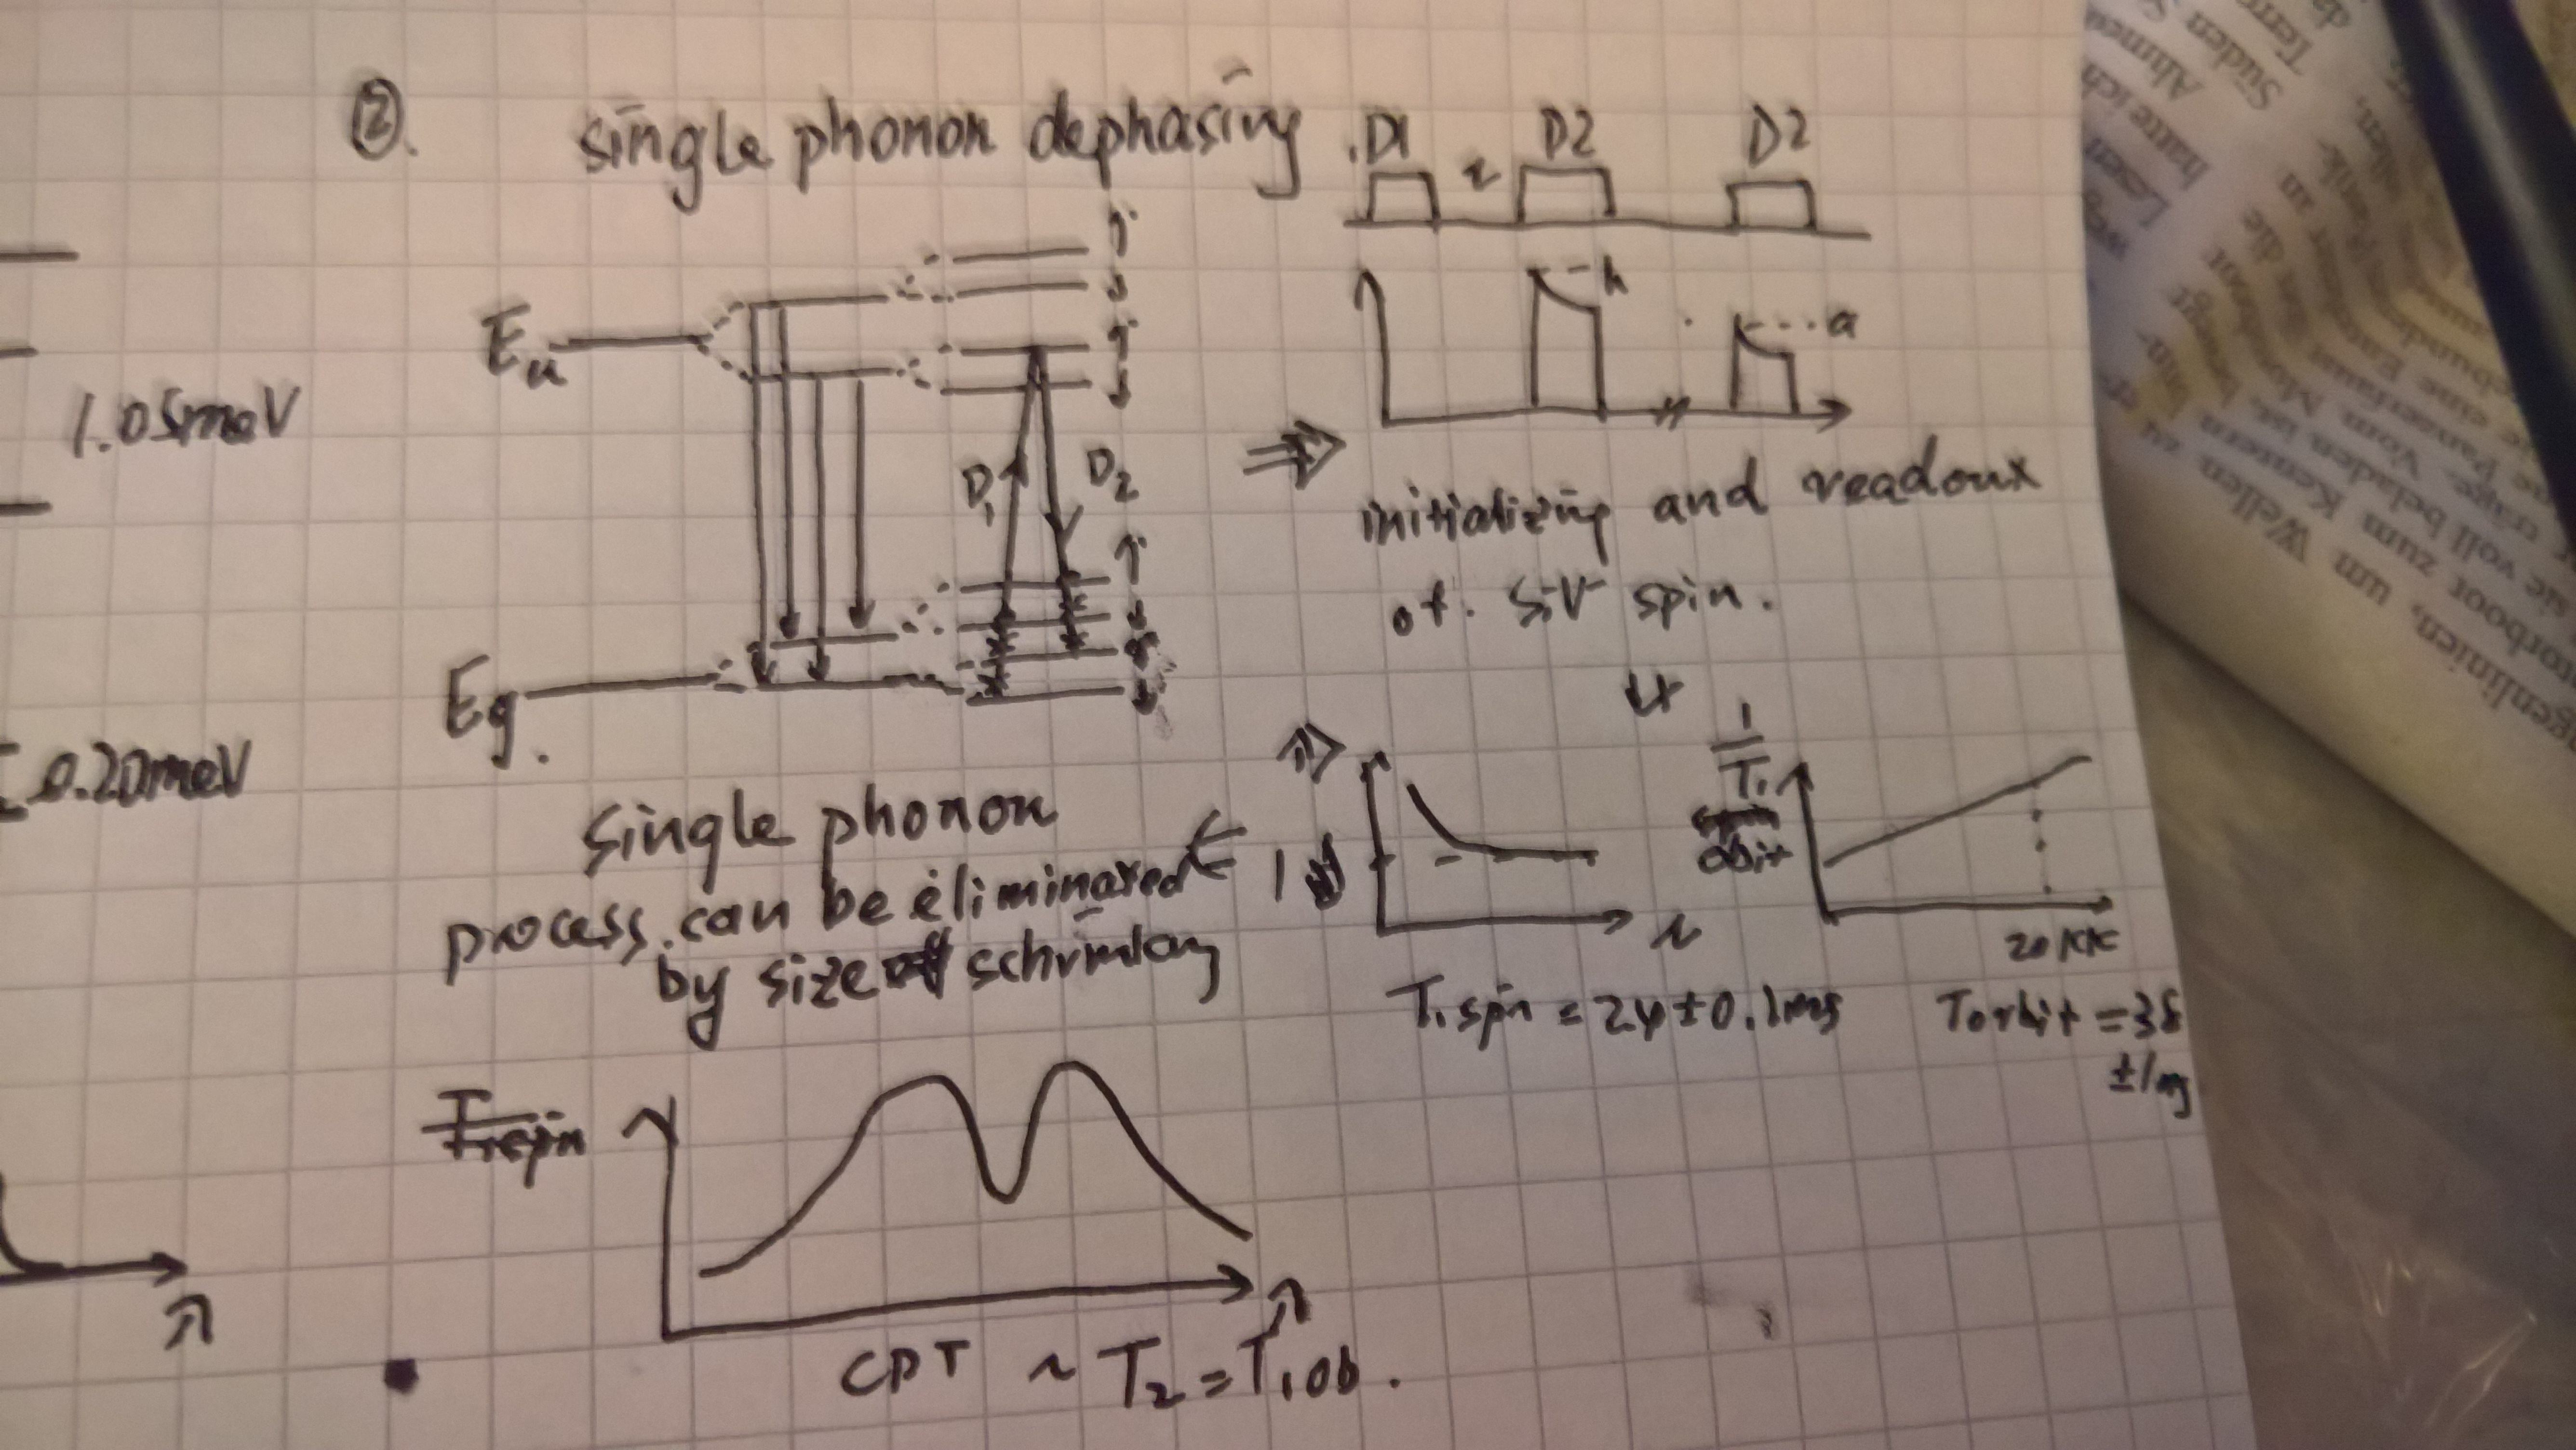
\includegraphics[width=1\linewidth]{Figures/pic/WP_20160921_20_40_32_Pro_LI}
\caption{}
\label{fig:wp20160921204032proli}
\end{figure}
\FloatBarrier

%----------------------------------------------------------------------------------------

\section[Silicon vacancies in nanodiamonds]{Silicon vacancies in nanodiamonds}
\FloatBarrier
\begin{figure}[h]
\centering
\includegraphics[width=1\linewidth]{Figures/pic/WP_20160921_20_40_48_Pro_LI}
\caption{}
\label{fig:wp20160921204048proli}
\end{figure}
\FloatBarrier
As mentioned, one vital problem to solve if we want to use SiV$^{-}$ as a qubit is that, the coherent time has been limited by the rapid orbital relaxation. And this is caused by the transition between the degeneracies of ground state which was driven by a single phonon. The elimination of such phonon is an direct approach towards the solution.

Spontaneous emission is inhibited if the cavity has characteristic dimensions which are small compared to the radiation wavelength [Daniel Kleppner1981]. As in our case to eliminate the emission of phonon that couples into the splitting of ground state in SiV$^{-}$ 47 GHz, nanodiamond of the size that is smaller than the half wavelength of this transition phonon wavelength (around 125nm) is desired. 

Currently 3 major techniques are employed in the field of nanodiamond fabrication: denotation, CVD, and HPHT, while the exotic atoms can be mixed in the beginning or implanted via ion implantation. While the denotation method produced highly defective diamonds and ion implantation introduces inner strain, for the SiV containing nanodiamonds, HPHT method and CVD method are the top choices.

The principle of CVD method is to disintegrate the CVD fabricated diamond film, while the HPHT method initialize an phase transition of carbon at high temperature and high pressure. Previously, comparison between the PL spectra of silicon doped polycrystalline diamond films obtained by the CVD method and diamond single crystals grown at a pressure of 6 GPa from a nickel melt at 1500$^{o}C$ has been carried out, and demonstrates that the HPHT diamonds carries narrower SiV$^{-}$ ZPL lines than CVD fabricated ones[C. D. Clark 1995]. As in the department of nanodiamonds, the narrowest SiV$^{-}$ ZPL that has been measued by far, which has the width that is almost of the excitation state life time limit, is also from the HPHT method fabricated nanodiamond.


 
\paragraph{Band-bending near the surface of diamond}  


%--------------------------------------------------------------------------------------

\section[Motivation of the thesis, unsolved problem]{Motivation of the thesis, unsolved problem}
\FloatBarrier
\begin{figure}[h]
	\centering
	\includegraphics[width=1\linewidth]{Figures/pic/WP_20160921_20_40_42_Pro_LI}
	\caption{}
	\label{fig:wp20160921204042proli}
\end{figure}
\FloatBarrier
The motivation of looking into SiV$^{-}$ in nanodiamonds is to acquire longer coherent time by eliminating the phonon that is responsible for the transition between the fine splitting of the ground state. Yet the obstacle on our way of justifying this approach is that, the optical properties of SiV$^{-}$ in nanodiamonds are not as outstanding as it is in bulk diamond. Blinking and spectral diffusion, especially spectral diffusion has stopped us from further life time measurement. 

The mechanism behind the spectral diffusion is yet not clear, our first guess is to connect the enhancement of spectral diffusion in nanodiamonds with the surface condition, due to the high surface to volume ratio of nanodiamonds.

Aerobatic oxidation can purify the nanodiamonds via the removal of Sp$^{2}$ phased carbon.
% Chapter 2
\chapter[Experimental approach of surpressing the spectral diffusion]{Experimental approach of surpressing the spectral diffusion} % Main chapter title

\label{Chapter2} % Change X to a consecutive number; for referencing this chapter elsewhere, use \ref{ChapterX}

%----------------------------------------------------------------------------------------
%	SECTION 1
%----------------------------------------------------------------------------------------
\section{Information regarding the nanodiamond sample}

\paragraph{here is a paragraph about the fabrication of nanodiamond}
\paragraph{here is a paragraph about the separation of the nanodiamonds}
\section[sample preparation]{sample preparation}
\subsection{preparation of the substrate}
\paragraph{IIa diamond as substrate}

To choose a proper substrate for the nanodiamond sample, a few principles need to be considered.

\paragraph{1.}Low background fluorescence. 
It is always vital to obtain a decent signal to noise ration in any kind of meansurements. As for our case, the emission(fluorescence) from sillicon centers are the target, thus we would love to lower the back ground fluorescence as much as possilble.
\paragraph{2.}Good heat conductivity at low temperature.
From previous calculation done by Uwen Jantzen, we know that the temperature difference $\bigtriangleup T$ between the bottom of the substrate and nanodiamonds(which are spin coated on the surface of the substrate) can be estimate as\newline
$\bigtriangleup T = \frac{\sigma \cdot d \cdot T^{4}}{k} $,
where $\sigma$ is the Stefan–Boltzmann constant, $d$ is the thickness of the substrate and $k$ is the thermal conductivity.
To resolve the fine feature of sillicon vacancy ZPL, we want to characterise the nanodiamond sample at a temperature that is lower than 30K for spectrometer and 10K? for PLE.
\paragraph{3.} No distracting spectral features.
Some misleading peaks from the emission of the substrate would be the least wanted when we want to character a sample spectrally. In many cases, this is related to the raman-scattering of the photons, which highly depends on the crystal structure of the substrate. This scattering process alters the energy of the incident photons by shifts of concrete values and sometime can introduce peaks that are misleading or distracting.
\paragraph{4.}Refractive index. Inam et al calculated the relative emission rate for radiating dipoles near an interface between two dielectrics with FDTD simulation. The result demonstrates that in both of the cases, when the dipole lies prependicular and parallel to the substrate, the emission rate from a interface with lower relative refractive index is always higher than that from a interface with higher relative refractive index. And to increase the emission rate, a substrate with lower refractive index would be prefered.
\paragraph{}Prevously, taking these principles into consideration, my colleges have already ruled out a couple of materials, for instance, glass/quartz(distraction raman shift lines) and Sapphire(also a distracting raman shift line, and impurity induced emission that calls for extra attention when picking the optical filters). Now the temporary choice has landed on IIa type diamond, which has a low impurity density(resulting in low background fluorescence intensity), relatively low refractive index(2,4 to 2,7), good thermal conductivity($\bigtriangleup T = 4,17 \cdot 10^{-2}K$) and a raman shift at 1332$cm^{-1} $ that causes no distraction on our observation.

\paragraph{Focused Ion Beam milling}
In order to make it more convenient to trace the nanodiamonds, markers were curved onto the surface of the IIa type diamond substrate, this work was done by Uwe Jantzen during his master's thesis period. As is shown in the fig.[], the focues ion beam bombards the surface of diamond away and leaves behind markers that are visible in optical microscopy images and SEM images, as well as confocal microscopy images.
\paragraph{here is a sketch of how Ga-ion bombards the surface of substrate}
\paragraph{here insert image of markers, optical, sem and confocal}
\paragraph{fig. ?.  }



\subsection{spin-coating of the sample}
\subsubsection{theory of spin coating} 
Spin coating is the method of sample preparing that mainly contains 2 steps:

1. Spreading of the liquid. In this step, certain volume of liquid containing the particle that we want to coat with is dropped on the surface of the substrate, driven by the centrifuging force from the rotational movement of the substrate, the liquid would be spread evenly on the surface.

2. Evaporation of the 'solvent'. While the sample stage rotates, the 'solvent'(In our case is not a real solvent, since nanodiamonds never really desolve.) would evaporate, leaving the particle/molecules that are wanted to be coated on the substrate.

In this procedure, 2 factors we find important.

1.spin speed: generally the thickness of the liquid layer $t$ is proportional to the inverse of the angular velocity $w$ squared t $\sim$ $\frac{1}{\sqrt{\omega}}$, higher speed would help with forming a more uniform layer, yet this also means a smaller volume of solution, which would lead to lower density of nanodiamonds of the surface. On the other hand, with lower speed, the probability of aggregation would increase, which is also what we want to prevent.

2.volume of the 'solution': larger volume means longer drying time, which would increase the probability of aggregation and losing nanodiamonds, while smaller volume leads towards lower density of nanodiamond and more difficulty when trying to drop it with a pipette. 

3.type of solvent: The type of solvent, viscosity and boiling point are important for the dispersion of nanoparticles inside solution, the spreading of the solution while spin coating and the rate of evaporation.

4.surface condition of the substrate. High contact angle is a obstacle towards the spreading of the solution, high roughness or inappropriate surface group of the substrate can result in poor wettability from the solution.

Throughout my project, with the help of Andrea Kurz, several combination of these factors had been has been tried out and in the end we landed on 

\paragraph{here we need a list of different program of spin coating that we have tried,with indexxxxx}

%-----------------------------------
\subsubsection{Acid cleaning}
To make sure that the NDs dispension can evenly spread and eventually settled on the substrate, a smooth, clean and hydrophilic surface is important.

Acid boiling is a very practicle way of diamond substrate cleaning. As it is called, the diamond will be boiled in a mixture of three strong mineral acids: sulfuric acid, nitric acid and perchloric acid. This mixture has ver strong ability of oxidizing.

\paragraph{here insert a sketch of how we do acid cleaning} 

After assembling the setup, we initialize the reaction by heating the mixture to a temperature where is mildly bubbles. The substrate would be stay inside the boiling tri-acid mix for 4h. 
The mixture of strong mineral oxidizing acid can remove most of the adhesions on the surface of diamond substrate , leaving a clean hydrphilic surface. This oxidizing procedure will lead to the formation of carbonyl and carboxyl groups.




\paragraph {here insert image of before and after cleaning substrate, optical image, confocal image }
fig. the comparision between before and after acid boiling.
 
Tri Acid boiling blabla. Expectation of the surface. Before after cleaning. Optical image. Confocal image.

%-----------------------------------
%	SECTION 2
%-----------------------------------
\section[development of a technology to estimate the spectral diffusion]{development of a technology to estimate the spectral diffusion}

\paragraph{Setup} 

In order to resolve the fine structure of ZPL of SiVs, we need to observe the sample at low temperature, thus a cryogenic setup must be applied.
Our setup is a typical confocal micropscopy setup connects with a cryostat, which cools the sample with liquid Helium flow.

\paragraph{here inserts a picture of our flow cryostat, from out and in side.}
This is the flow cryostat, whose main body is a vaccum chamber with

\paragraph{here insert a sketch of the cryo4 setup}
Confocal + Cryostat, Green laser + Red laser, spectrometer, apd, pic


\paragraph{PL} Photoluminescence spectra is one of the most efficient way of finding silicon vacancies. In this measurement, we use green laser of 532nm to excite the Silicon vacancies from ground state to 

\paragraph{PLE} resonance excitation of optical transition. Rsésolution limited by scanning step of laser. Observing phonon side band with apd. range of scanning: limited by laser, small.

\paragraph{time resolved PL spectra} Tracing PL spectra over time, show the diffusing behaviour of lines, characterisation methods: excitation polarisation: width of diffusion. Cross- correlation over time.
\paragraph{}We recorded and noticed that the diffusion, whose range can up to 1nm, is far beyond the capability of PLE. 

%-----------------------------------
%	SECTION 3
%-----------------------------------
\section{Oxidation}
\paragraph{Effect of Oxidation}
Room temperature oxidization is a common way of nanodiamond purification. With different oxidizing temperature, different types of impurities can be removed from the surface of the nanodiamond, ranging from water and physisorbed organic impurities, amourphous carbon, and graphitic shells and ultimate the $sp^{3}$ phase of diamond[T.Gaebel,2010]. After the oxidation, carbonyl and carboxyl groups are formed on the surface[Petrakov,2012]. Several paper have mentioned temperature choices for oxidation aiming at impurity removal. During the master's thesis period, 2 different oxidation has been examined.

\subsection[first Oxidation]{first Oxidation}
\paragraph{method}As reported, oxidation of $sp^{2}$ carbon already starts at $400^{o}C$, while the size reducing rate of diamond phase remains neglactable when the temperature is lower than $500^{o}C$. So it is an obvious choice to settle down the oxidation temperature at somewhere close to $500^{o}C$ when the maximum removal of $sp^{2}$ phased carbons and the minimum lost of the diamond body($sp^{3}$ phased carbons). Inspired by Elka Neu's paper, ....here insert a sentence explaining why we choose the two step oxidation program.
\paragraph{setup}

The aerobatic oxidation is carried out in a tube furnace that is offered by the ?? institute and it is done with the help of Markus Mohr. The tube furnace consists of a glass tube connected to the room atmosphere and heating coils around the glass tube. The glass tube is slidable. We put our sample inside a ceramic ?bowl? and put the bowl into the glass tube carefully, after the temperature has been raised to ?460C?, the glass tube would be slide into the heating coils. After the Oxidation, the glass tube would be slide out and the sample would cooled inside the tube until room temperature.

\paragraph{pre-characterisation}
Before the oxidation, we tried to characterise the sample with several different methods based on our confocal microscopy setup.

1. RT imaging and PL spectra

First we take a scan with green laser and record the fluorescence with an APD, which offers us a confocal microscopy image of the surface of the sample, then the photoluminescnce spectra of the bright spots are taken, those ones with a sharp peak at 737nm are saved as points of interests and their positions are saved as region of interest for the reference of further examine.

2. Cold spectra and PLE 
The sample is attached to an cold finger and the placed inside the cryostat, after UHV condition has been achieved, we start the helium transfer, which would brought the temperature of the sample down to 4.8K. We refound the points of interests that has been confirmed with SiV like spectra

3. PLE spectra

4.time-resolved PL spectra.

\paragraph{post-oxidation characterisation}
1. Optical microscopy check
The first thing we found after the oxidation is that, the surface of our sample turned very dirty. We are yet not certain about what the contaminations are, are they intrinsic or are they external. A possible deduction is that, the contamination comes from the glass tube of tube furnace, that the residues of previous treatments has attached to the inner surface of the tube and evaporized again, depositing on the surface of our sample. Further improvement of oxidation operation has been done in our second oxidation test, and will be mentioned in the next part of the thesis.


2. confocal microscopy imaging and PL spectra.
Huge amount of bright spots can be seen in the confocal image when we excite the sample with 532nm green laser. There's no Silicon vacancy like spectra found in these bright spots. We refind our points of interests next to the marker 4C. The photoluminescence spectra shows much higher intensity than before the oxidation.


3. Cold spectra and PLE 
After the confirmation of points of interests, the sample was transfered into the flow cryostat and the helium flow brought the temperature down to 4.8K.

At 4.8K we recorded the time-resolved photoluminescence spectra of different incident beam power with an excitation wavelength of 532nm. 

After the first oxidation, we learned that due to the inner strain of photonic fibre, the incident beam can not preserve a static polarisation. To stable the polarisation, we used a polarising beam spliter with a LC noise eater behind it. This would fix the polarisation at vertical direction.


\paragraph{Analysis}

\subsection[Second Oxidation]{second Oxidation}

\paragraph{method} As is mentioned before, the optical properties of SiV in bulk diamond is extraordinary. Most importantly, the spectrodiffusion that we have observed in nanodiamonds has never been seen in bulk diamonds. In the first oxidation, it seems the removal of graphitic impurity didn't help with the stablization of emiision lines. In this second oxidation, we decided to used a higher temperature to acquire a surface with groups that imitates the bulk diamond.As reported by [paper], after 2 hours of aerobatic oxidation at $575^{o}C$, ... here insert a sentence of the surface groups of nanodiamonds. To increase the chance of finding smaller nanodiamonds that would fit into a cavity and decrease the chance of getting clusters of nanodiamonds, this time we chose to use nanodiamond of the first batch. These nanodiamond are spin coated on the substrate following the method II(the index, can be change).

Taking the experiences of last oxidation into consideration. This time we introduces flowing inert gas (helium) to flush away the potential contaminations during the cooling process. This can also prevent the result to be affected by the humidity of the air.
We found out the extinction rate of polarising beam spliter is not ideal, so this time we used a Clan Thompson polarisation filter instead.
\paragraph{Before Oxidation}
1.Optical microscopy observation
  
We observed the sample after the spin coating with optical microscopy, the surface appeared to be relatively clean, little amount of contamination has been observed, but is acceptable.

2.Mapping of $SiV^{-}$ with room temperature setup.

Once again, we exxplored the sample with the same room temperature confocal microscopy setup. With the help of spectrometer, we find a few points of interest with a emission spectrum that resembles $SiV^{-}$. 

3. Cold time resolved PL and exitation polarisation

As has been mention in last chapter, it is suspect that the incident polarisation can affect the spectral behaviour of SiV. We added in the excitation polarisation measurement and recorded the time resolved photoluminescence spectra of 2 different excitation polarisation that are perpendicular to each other. This is achieved by putting a motor-driven half-lambda plate after the noise eater. 
Due to short time scheme from this measurement we decided to fix the input power at [?need to check], which is the lowest power that can offer most of the points of interest's a decent signal to noise ration.




\paragraph{After Oxidation} 

1. Optical Microscopy observation. 

After the Oxidation, we found the surface not as dirty as the last Oxidation. It seems a cleaner tube and flowing gas flushing do have helped suppressing the surface contamination introduced by the tube furnace.



\paragraph{Analysis} 
Comparasion if possible: different behaviour pre treatment between two batches
Possible reason: losing NDs due to Helium flow while cooling, GR1 getting closer to the surface due to oxidation caused size/thickness reduction.

%----------------------------------------------------------------------------------------
%	SECTION 4
%----------------------------------------------------------------------------------------

\section[H termination]{H termination}
\paragraph{Effect of H termination}

NEA, band structure of diamond. Reduction of surface.
\paragraph{method} Plasma treatment, setup, apparatus.

\paragraph{why no pre characterisation} Conditions for Plasma treatment.

\paragraph{After H termination} Confocal image, optical image, excitation polarisation, time resolved PL with different incident polarisation.


\paragraph{Analysis} Within the instrumental limit of spectrometer, the spectral diffusion has been significantly suppressed. Possible reason. 
\chapter{Conclusion and outlook} % Main chapter title

\label{Chapter3} % Change X to a consecutive number; for referencing this chapter else where, use \ref{ChapterX}
%----------------------------------------------------------------------------------------
%	SECTION 1
%----------------------------------------------------------------------------------------

\section{Conclusion}

In the thesis we characterised spectrally the SiV$^{-}$ in nanodiamonds of 2 different size distributions with the help of confocal microscopy at cryogenic temperature. It has been noticed that the untreated SiV$^{-}$ in nanodiamonds are spectrally not stable, and SiV$^{-}$ smaller diamonds have worse spectral stability than larger ones. This spectral diffusion can be resolved in PL spectra. Previously it has been shown that the surface charging state plays a vital role in color centre luminescence. Negative charges on the surface can lead to depletion of NV \citep{stacey_depletion_2012}. For nanodiamonds, the band bending which originates from the difference of chemical potential in the bulk and on the surface is closely related to size-effect relating phenomena. It is highly suspected that the spectral diffusion of SiV$^{-}$ in nanodiamonds is also surface charge related.

Large number of PL spectra were taken to trace drift of lines. A standard method for spectral stability has been put forward. The calculation of mean cross-correlation can conclude the similarity of spectra into one number ranging from 0 to 1, Which makes statistical comparison possible. At the same time, time-resolved spectra realises the visualisation of spectra diffusion by plotting spectra over time in to colour maps.

Three surface treatment has been employed to modify the surface charging property. Aerobic Oxidation at 460$^{o}C$ - 480$^{o}C$ was used to selectively remove the graphitic defects on the surface while mild oxidation, resulting in carbonyl and carboxyl groups covered surface. Elevated temperature oxidation (575$^{o}C$) was used to initialize a bulk-diamond-like surface structure. Hydrogenation was to form a surface that posses negative electron affinity.

The oxidation at elevated temperature didn't produce useful data due to the distraction of substrate. The mildly oxidized sample showed heavily enhanced luminescence and worse spectral stability while the hydrogen terminated sample showed slightly reduced luminescence intensity and improved spectral stability.

%-----------------------------------
%	SECTION 2
%-----------------------------------
\section{ Outlook}

\paragraph{PL and PLE}
It is suspected that the ionization of Nitrogen atoms has been involved in the process, it is interested to compare the time-resolved spectra excited with a 532nm laser and a laser of 730nm.

PLE characterisation of the sample with improved spectra stability is also attractive, with reduced spectral diffusion, it might be finally possible for us to resolve the 4 line structure of SiV$^{-}$ ZPL.

\paragraph{life time measurement}
Due to the spectral diffusion, the orbital T1 measurement of untreated sample was not able to be carried out. With the improved spectral stability (need to be proved by PLE first), it might become possible. A longer time life will offers more possibility on the development of SiV$^{-}$ qubit.

\paragraph{Surface treatments}

Different surface treatments and comparison can help us understand the mechanism of spectral diffusion better. The most convenient treatments now are the hydroxylation which can be carried out directly on the hydrogenated sample resulting in a transform from negative electron affinity to positive electron affinity of the surface.

Anther interesting treatment is the dehydrogenation of sample by vacuum annealing, as the temperature varies, this can result in a clean diamond surface or a surface covered with thin-thick layer of graphite, which results in a gradual change in the surface electron affinity. \citep{diederich_electron_1998,maier_electron_2001}

Aerobic Oxidation still has more possibility to deal with. Since the size reduction rate of certain temperature is known, it is possible to profile the size effect on spectral stability by decreasing the size of nanodiamonds via oxidation gradually. It can also used to treat nanodiamonds that are too large (batch3, 4) for phonon elimination. The oxidation can also help to separate aggregated diamonds.

\paragraph{better method for size selection}
It is noticed, the size selection via centrifugation works, but is quite coarse. It might be possible to obtain finer batches by methods like high performance liquid chromatography. \citep{naoki_komatsu_chromatographic_2011}

\paragraph{relation between surface geometry and spectral behaviour}
Since it is possible to obtain the excitation polarisation pattern, it is interesting to observe the orientation preference of SiV$^{-}$/nanodiamonds statistically. This can be related to the formation process of HPHT diamond.



%----------------------------------------------------------------------------------------
%	THESIS CONTENT - APPENDICES
%----------------------------------------------------------------------------------------

\appendix % Cue to tell LaTeX that the following "chapters" are Appendices

% Include the appendices of the thesis as separate files from the Appendices folder
% Uncomment the lines as you write the Appendices

% Appendix A

\chapter{Appendix Title Here} % Main appendix title

\label{AppendixA} % For referencing this appendix elsewhere, use \ref{AppendixA}

Write your Appendix content here.
%\include{Appendices/AppendixB}
%\include{Appendices/AppendixC}

%----------------------------------------------------------------------------------------
%	BIBLIOGRAPHY
%----------------------------------------------------------------------------------------

\printbibliography[heading=bibintoc]

%----------------------------------------------------------------------------------------

\end{document}  
